\documentclass[a4paper,11pt,oneside,openany,article]{memoir}
\usepackage[fleqn]{amsmath}
\usepackage{amsthm}
\usepackage[english,dutch]{babel}
\selectlanguage{dutch}
\usepackage[fixlanguage]{babelbib}
\selectbiblanguage{dutch}
\usepackage{enumitem}
\usepackage{float}
\usepackage{graphicx}
\usepackage[colorlinks,linkcolor=black,citecolor=black,filecolor=black,urlcolor=black,hypertexnames=false,naturalnames=false]{hyperref}
\usepackage{mathtools}
\usepackage{rotating}
\usepackage{tikz}
\usepackage{xspace}

% must come after hyperref
\usepackage[capitalise,dutch]{cleveref}
\crefname{figure}{Figuur}{Figuren}
\crefname{section}{Hoofdstuk}{Hoofdstukken}
\crefname{subsection}{Hoofdstuk}{Hoofdstukken}

% colors
\definecolor{uablue}{RGB}{0,61,100}
\definecolor{uared}{RGB}{126,0,47}
\definecolor{vividbrown}{RGB}{215,154,70}
\definecolor{uagreen}{RGB}{0,126,17}

\usetikzlibrary{matrix,arrows}

% memoir tweaking
\renewcommand{\thesection}{\arabic{section}}

% babelbib sucks
\declarebtxcommands{dutch}{%
  \def\btxnumeralshort#1{%
    \btxnumeralenglish{dutch}{#1}}%
  \def\btxnumerallong#1{%
    \ifnumber{#1}{%
      \ifcase#1 nulde\or eerste\or tweede\or derde\or
        vierde\or vijfde\or zesde\or zevende\or
        achtste\or negende\or tiende\else
        \btxnumeralenglish{dutch}{#1}%
      \fi}{#1}}%
}

% fonts
\usepackage[T1]{fontenc}
\usepackage[charter]{mathdesign}
\usepackage[scaled]{beramono,berasans}
\usepackage{microtype}
\frenchspacing

\addtolength\headheight{12pt}
\addtolength\parskip{.7ex}
\setlength\parindent{0cm}

\relpenalty=10000
\binoppenalty=10000

\theoremstyle{definition}
\newtheorem{theorem}{Stelling}
\newtheorem{lemma}[theorem]{Lemma}
\newtheorem{corollary}[theorem]{Gevolg}
\newtheorem{definition}[theorem]{Definitie}
\newtheorem{example}[theorem]{Voorbeeld}
\newtheorem{remark}[theorem]{Opmerking}
\crefname{theorem}{Stelling}{Stellingen}
\crefname{lemma}{Lemma}{Lemma's}
\crefname{definition}{Definitie}{Definities}
\crefname{example}{Voorbeeld}{Voorbeelden}
\crefname{remark}{Opmerking}{Opmerkingen}

\newtheorem*{exercise}{Exercise}
\newenvironment{solution}[1][\textbf{Solution}\hspace{1em}]{#1}{\hfill\qed}

% http://tug.org/pracjourn/2006-3/robertson/robertson.pdf
\newcommand\foreign[1]{\emph{#1}}
\newcommand\eg{\foreign{e.g.}}
\newcommand\Eg{\foreign{E.g.}}
\newcommand\ie{\foreign{i.e.}}
\newcommand\Ie{\foreign{I.e.}}
\newcommand\vs{\foreign{vs.~}}
\newcommand\cf{\foreign{cf.\@}}
\newcommand\resp{\foreign{resp.\xspace}}
\newcommand\etc{\foreign{etc.}}
\newcommand\etal{\foreign{et al}}

\newcommand\betti{\mathrm{b}}
\newcommand\Dih{\mathrm{Dih}}
\newcommand\eulercharacteristic{\chi}
\newcommand\fundamental{\homotopyGroup_1}
\newcommand\Grp{\mathsf{Grp}}
\newcommand\homologyGroup{\mathrm{H}}
\newcommand\homotopyGroup{\pi}
\newcommand\poincare{\mathrm{P}}
\newcommand\PCat{\mathsf{Psh}}
\newcommand\SCat{\mathsf{Sh}}
\newcommand\sections{\mathrm{\Gamma}}
\newcommand\Sets{\textsf{Sets}}
\newcommand\ShfSpace{\mathrm{L}}
\newcommand\Shf{\mathrm{\Gamma}}
\newcommand\sphere{\mathbb{S}}
\newcommand\TopP{\mathsf{Top}_{\bullet}}
\newcommand\torus{\mathbb{T}}

\DeclareMathOperator\Coker{Coker}
\DeclareMathOperator\Hom{Hom}
\DeclareMathOperator\identity{id}
\DeclareMathOperator\Image{Im}
\DeclareMathOperator\Ker{Ker}
\DeclareMathOperator\Ob{Ob}

\selectlanguage{english}

\begin{document}
\selectlanguage{english}
\title{\textls[20]{Solutions to Tennison}}
\author{
  Pieter Belmans
}
\maketitle

\tableofcontents*

\chapter{Solutions to the exercises at the end of Chapter 1}
\begin{enumerate}
  \item Prove that the~$\varinjlim$ of the direct systems of the examples is~$F(\emptyset)$ in each case. Generalise.

    \begin{solution}
      The direct system of a topology corresponds to a complete lattice, hence there is a minimum and a maximum: $\emptyset$ and~$X$. The direct limit now corresponds to `the object that goes to the right of everything' but in this case,~$\emptyset$ is on the right over everything, therefore, the direct limit is given by~$F(\emptyset)$.
    \end{solution}

  \item Prove directly from the definitions that if~$U$ is a direct limit of a direct system~$(U_\alpha)_{\alpha\in\Lambda}$ of sets, then~$U=\bigcup_{\alpha\in\Lambda}\Image(U_\alpha\rightarrow U)$.

    \begin{solution}
      The~$\rho_{\alpha,\beta}$ in the definition of a target are injective maps. Now the set~$\coprod_{\alpha\in\Lambda}U_\alpha$ is a possible target, with~$\sigma_\alpha$ mapping an element to all positions in the disjoint union such that it is contained in the corresponding set~$U_\gamma$.

      By the definition of the direct limit, there must be a unique~$f$ to this target, making the triangle commute. But as I'm writing this, it feels like a reformulation of Theorem~3.10.
    \end{solution}

  \item
    \begin{enumerate}
      \item Interpret and prove: a set is the direct limit of its finite subsets.
      
        \begin{solution}
          The construction of the direct limit consists of quotienting the disjoint union. All elements of the set~$U$ are represented in a finite subset (for instance the singletons), so the disjoint union contains all elements. Elements are now identified if they are identified in the power set lattice of~$U$, but as the union of two finite subsets is still finite the identification of an element~$v\in U_\alpha,U_\beta$ occurs in~$U_\gamma=U_\alpha\cup U_\beta$.
        \end{solution}

      \item Interpret and prove: an abelian group is the direct limit of its finitely generated subgroups.

        \begin{solution}
          Analogously, finitely generated subgroups are represented in the same kind of lattice structure with atoms and finite unions of generators. 
        \end{solution}

      \item Can you obtain~$\mathbb{Z}$ as a direct limit of finite abelian groups?

        \begin{solution}
          No, only torsion groups are obtainable. As finite abelian groups are all isomorphic to products of~$\mathbb{Z}/p\mathbb{Z}$ and we'll be taking a quotient from a direct sum, all elements will keep their finite order.
        \end{solution}
    \end{enumerate}

  \item
    \begin{enumerate}
      \item Characterise direct systems of sets with~$\varinjlim=\emptyset$.

        \begin{solution}
          As the direct limit consists of the disjoint union modulo some relations, the direct limit is always nonempty, \emph{unless} the disjoint union itself consists of empty sets. Therefore all sets in the direct system must be empty: you cannot obtain an empty quotient from a nonempty set.
        \end{solution}

      \item Produce an interesting direct system of abelian groups with~$\varinjlim=\left\{ 0 \right\}$, the trivial group. Characterise such systems.

        \begin{solution}
          As the construction of the direct limit consists of taking the direct sum of all groups and taking the quotient with the subgroup generated by all~$\inj_\alpha(g_\alpha)-\inj_\beta(\restr_{\alpha,\beta}(g_\alpha))$ we need to obtain \emph{all} elements of the direct sum. Hence~$\inj_\beta(\restr_{\alpha,\beta}(g_\alpha))$ must be zero for all~$(\alpha,\beta)\in\Lambda_1$. So~$\restr_{\alpha,\beta}$ must kill all elements, we therefore have rather boring restriction morphisms.
        \end{solution}
    \end{enumerate}

  \item What can you say about the direct limit of a direct system all of whose maps are injective? Surjective?

    \begin{solution}
      All the maps to the direct limit are injective (or surjective). In the injective case the direct limit contains information on~\emph{all} objects of the direct system, in the surjective case the direct limit contains the~\emph{common} information of all objects.
    \end{solution}

  \item For~$n\in\mathbb{N}_0$, let~$C_n(x)$ denote a cyclic group of order~$n$ with generator~$x$. Let~$p\in\mathbb{N}$ be a prime number. Let~$G$ be the direct limit of the following direct system of abelian groups:
    \begin{equation}
      \left\{ 0 \right\}=C_{p^0}(x_0)\rightarrow C_{p^1}(x_1)\rightarrow\ldots\rightarrow C_{p^n}(x_n)\rightarrow C_{p^{n+1}}(x_{n+1})\rightarrow\ldots
    \end{equation}
    (where~$C_{p^n}(x_n)\rightarrow C_{p^{n+1}}(x_{n+1})$ takes~$x_n\mapsto px_{n+1}$). Preferably without resorting to the explicit construction prove:
    \begin{enumerate}
      \item $G$ is infinite, but torsion (\ie~element has finite order).

        \begin{solution}
          Based on the previous exercise we realize that~$G$ is a big structure as every map is injective. As every step in the chain adds a finite number of elements and there are countable steps, we obtain a countable infinite group.

          As the construction of the direct limit consists of summing all objects of the direct system and taking a quotient, we get that every element of the direct sum has finite order (namely the order of the highest term) and the quotient keeps this structure.
        \end{solution}

      \item Every finitely-generated subgroup of~$G$ is finite. Find all of them.

        \begin{solution}
          Every finite set of generators has a maximal index~$n$ such that the term for~$C_{p^n}$ is nonzero but for~$C_{p^{n+1}}$ is zero. The order of the finitely-generated subgroup is now limited by the order~$p^n$.
        \end{solution}
    \end{enumerate}

    Deduce that~$G$ has no proper infinite subgroup, and no maximal proper subgroup. Can either of these situations arise for subspaces of a vector space (using dimension instead of order)? Identify a realisation of~$G$ inside the unit circle~$S^1\subseteq\mathbb{C}$ (under multiplication).

    \begin{solution}
      The construction of the direct sum learns us that there must be an infinite number of nonzero summands, but as every~$C_{p^n}$ is trivially embedded in~$C_{p^m}$ for all~$m>n$ and every such instance is identified we cannot get to a proper infinite subgroup. Analogously there is no maximal proper subgroup.

      The only interesting case occurs in infinite-dimensional vector spaces, the finite-dimensional case is trivial (take the quotient of the space with the field).

      The obtained structure is the Pr\"ufer group.
    \end{solution}

  \item Consider the following direct system of abelian groups: fix~$r\in\mathbb{Z}$; for all~$n\in\mathbb{N}$ let~$U_n=\mathbb{Z}$ and for~$n\geq m$ let~$\rho_{m,n}\colon U_m\to U_n$ be multiplication by~$r^{n-m}$. Identify the~$\varinjlim$ as a subring of~$\mathbb{Q}$.

    \begin{solution}
      This is the localization at the ideal generated by~$r$. In the case of~$r$ prime this is~$\mathbb{Z}_{(p)}$, in the other case we obtain all fractions with prime factors of~$r$ as denominators.
    \end{solution}

  \item Interpret and prove: the direct limit of a system of exact sequences is exact.

    \begin{solution}
      For~$0\to A_n\to B_n\to C_n\to 0$ an exact sequence all the maps described in the definition of a direct limit are commuting by the properties of injective and surjective maps.
    \end{solution}

  \item The notions of target and direct limit can be formulated without the restriction (a) of Definitions~3.1 and~3.11. What difference does this make to the constructions? Find a system of abelian groups (in this generalised sense) with direct limit~$A\oplus B$ without having this abelian group appear in the system. Justify Remark~3.21.

    \begin{solution}
      Take~$X\colonequals]0,1[\cup]1,2[$ and the Euclidean topology with~$X$ removed from the topology. Now the direct system doesn't satisfy the conditions, but by taking a direct system on~$]0,1[$ that produces~$A$ as its direct limit (in the former sense) and likewise on~$]1,2[$ one that produces~$B$ we obtain a system of abelian groups in the generalised sense that produces~$A\oplus B$.
    \end{solution}

  \item Formulate the dual notions of inverse system and inverse limit~$\varprojlim$ (reverse the arrows).

    \begin{solution}
      As the exercise suggests, this is just a reversal of the arrows~$\rho_{\alpha,\beta}$ to~$U_\beta\to U_\alpha$, for~$\alpha\leq\beta$.
    \end{solution}
    
    Find inverse systems:
    \begin{enumerate}
      \item of finite sets whose~$\varprojlim$ is infinite;

        \begin{solution}
          Take~$(\mathbb{N},\leq)$ and define~$A_k=\left\{ 0,\ldots,k \right\}$. We get~$\rho_{i,j}\colon A_j\to A_i$ the projection for~$i\leq j$. The direct limit is the set~$\mathbb{N}$.
        \end{solution}

      \item of finite abelian groups whose~$\varprojlim$ is infinite;

        \begin{solution}
          The ring of $p$\nobreakdash-adic integers~$\mathbb{Z}_p$ is given by~$\varprojlim\mathbb{Z}/p^n\mathbb{Z}$.
        \end{solution}

      \item of abelian groups whose~$\varprojlim$ is~$\mathbb{Z}$ (without~$\mathbb{Z}$ in the system).

        \begin{solution}
          Start from~$\mathbb{Q}$. Let~$p_n$ denote the~$n$th prime number. Now define~$G_k$ to be the subgroup of~$\mathbb{Q}$ in which all primes but~$p_1,\ldots,p_n$ are allowed as factors of the denumerator. The morphisms are the injections. Now~$\mathbb{Z}$ is the inverse limit, it being the subgroup of~$\mathbb{Q}$ in which all prime factors of denumerators are removed.
        \end{solution}
    \end{enumerate}

  \item Verify that if~$(R_\alpha)_{\alpha\in\Lambda}$ is a direct system of abelian groups such that each~$R_\alpha$ is a ring and all the~$\rho_{\alpha,\beta}$ are ring morphisms, then~$\varinjlim R_\alpha$ has a natural ring structure such that all the maps~$R_\beta\to\varinjlim R_\alpha$ are ring morphisms.

    \begin{solution}
      The ring structure is preserved by the direct sum construction of the direct limit of abelian groups. As the subgroup~$H_1$ is the construction is an ideal because the multiplicative structure is preserved by the injections, we obtain a quotient ring.
    \end{solution}

  \item What are the stalks of the presheaf~$P_2$ of~2.E?

    \begin{solution}
      We have~$(P_2)_{x_0}=\mathbb{Z}$ as every open subset~$U$ containing~$x_0$ has~$P_2(U)=\mathbb{Z}$, with~$\rho_{\alpha,\beta}=\identity_{\mathbb{Z}}$ in the direct system.

      For~$(P_2)_{x}$ with~$x\neq x_0$ we get~$\left\{ 0 \right\}$, the trivial group. We have~$|x-x_0|=\epsilon>0$, so for the open set~$B(x,\epsilon)\cap[0,1]$ the presheaf gives~$\left\{ 0 \right\}$, all values of the presheaf from there on are the same trivial group.
    \end{solution}

  \item Construct a topological space~$X$ and a presheaf~$F$ of abelian groups on~$X$ with the properties:
    \begin{enumerate}
      \item for any open~$U\subseteq X$: $F(U)\neq\left\{ 0 \right\}$;
      \item for all~$x\in X$ the stalk~$F_x=\left\{ 0 \right\}$.
    \end{enumerate}
    If you cannot, prove that it is impossible. Compare with~4(b).

    \begin{solution}
      An interesting case with non-abelian groups would be to take the space~$X=[0,1]\cap\mathbb{Q}$ and assign to an open subset~$U$ the permutation on its elements. The direct limit is now the permutation on a single element, hence the trivial group.

      This is impossible, exactly by~4(b). We'd need restriction maps restricting everything to zero, but by the sheaf conditions this is impossible.
    \end{solution}
\end{enumerate}

\clearpage

\chapter{Solutions to the exercises in Chapter 2}
\begin{exercise}[1.9]
  Show that if~$G$ is an abelian sheaf, then~$G(\emptyset)=\left\{ 0 \right\}$, the trivial group.

  \begin{solution}
    By taking the empty cover of the empty set, the first part of the sequence that corresponds to the equalizer diagram reduces to
    \begin{equation}
      0\to G(\emptyset)\to 0
    \end{equation}
    because we're taking the product over an empty set ($\Gamma=\emptyset$). Now~$G(\emptyset)$ is embedded in~$0$, and must therefore be equal to the trivial group.
  \end{solution}
\end{exercise}

\begin{exercise}[1.12]
  Find an example with~$G$ not a monopresheaf where~1.10 fails.

  \begin{solution}
    Take both~$F$ and~$G$ the presheaf~$P_1$ from~Example~1.2.E. Now define~$f\colon F\to G$ to be the trivial map for~$F(U)\to G(U)$,~$U\neq X$ open and let~$f(X)\colon F(X)\to G(X):n\mapsto 2n$. Similarly,~$g(X)\colon F(X)\to G(X):n\mapsto 3n$. Now~$f$ and~$g$ agree on all stalks but as the monopresheaf fails (all restrictions are elements of the trivial group but the global behaviour differs) we have~$f\neq g$.
  \end{solution}
\end{exercise}

\begin{exercise}[3.7]
  Check the functorial properties
  \begin{equation}
    \left\{
      \begin{aligned}
        \sections(f\circ g)&=\sections f\circ\sections g \\
        \sections(\identity)&=\identity
      \end{aligned}
    \right.
  \end{equation}

  \begin{solution}
    We have a morphism of sheaf spaces~$\identity\colon E\to E$, obtaining a morphism of sections~$\sections(U,E)\to\sections(U,E):\sigma\mapsto\identity\circ\sigma$, which is locally an identity. This extends to the entire sheaf~$\Shf(E)$, so~$\Shf(\identity)=\identity$.

    As~$\Shf(g\circ f)$ is defined locally as a morphism of sections
    \begin{equation}
      \sections(U,E)\to\sections(U,E''):\sigma\mapsto g\circ f\circ\sigma
    \end{equation}
    in which~$f\circ\sigma\in\sections(U,E')$ by definition of~$\Shf(f)$, we obtained the desired property.
  \end{solution}

  Check also that if~$f\colon E\to E'$ is a morphism of sheaf spaces over~$X$, then
  \begin{equation}
    \left( \sections f \right)_x\colon\left( \sections E \right)_x\to\left( \sections E' \right)_x
  \end{equation}
  and
  \begin{equation}
    f|_{p^{-1}(x)}\colon p^{-1}(x)\to p'^{-1}(x)
  \end{equation}
  are isomorphic maps.

  \begin{solution}
    This is nothing but Proposition 3.6.
  \end{solution}
\end{exercise}

\begin{exercise}[3.9]
  Check the functorial properties

  \begin{equation}
    \left\{
      \begin{aligned}
        \ShfSpace(f\circ g)&=\ShfSpace f\circ\ShfSpace g \\
        \ShfSpace(\identity)&=\identity
      \end{aligned}
    \right.
  \end{equation}

  \begin{solution}
    The map~$\identity_x\colon F_x\to F_x$ is applied for all~$x$ and~$\ShfSpace(F)$ is the disjoint union of these stalks, so~$\ShfSpace(\identity)=\identity$.

    The composition is handled as in~$\Shf(f\circ g)$.
  \end{solution}
\end{exercise}

\clearpage

\chapter{Solutions to the exercises at the end of Chapter 2}
\begin{enumerate}
  \item Let~$I=[0,1]\hookrightarrow\mathbb{R}$. Show that there is a unique (up to isomorphism) sheaf~$F$ on~$I$ with stalks: $F_0=F_1=\mathbb{Z}$, $F_x=\left\{ 0 \right\}$ if~$x\in I\setminus\left\{ 0,1 \right\}$.

    \begin{solution}
      A presheaf has a unique sheafification, so we need to define a presheaf with these stalks and sheafify it. Do this by letting~$\sections(U,E)=\mathbb{Z}$ if~$\left\{ 0,1 \right\}\cap U\neq\emptyset$ and~$\sections(U,E)=\left\{ 0 \right\}$ otherwise. Now the stalks agree and~$\Shf(E)=F$.
    \end{solution}

    What is~$\Shf(I, F)$?

    \begin{solution}
      It is~$\mathbb{Z}\oplus\mathbb{Z}$, as it is composed of contributions of the stalks in~$0$ and~$1$.
    \end{solution}

    Let~$G$ be the constant sheaf~$\mathbb{Z}$ on~$I$. How many morphisms are there from~$F$ to~$G$? From~$G$ to~$F$?

    \begin{solution}
      To make the triangle in the definition of a (pre)sheaf morphism commute, observe that~$\restr_V^U$ is either the identity\footnote{Or some isomorphic map, the image of~$1$ defines the entire morphism and every morphism corresponds to a multiplication with a scalar.} of the projection on~$\left\{ 0 \right\}$ while~$\restr'{}^U_V$ is the identity for all open sets. So for a morphism from~$F$ to~$G$ we have on option: the identity on~$U$ containing~$0$ or~$1$ and the canonical injection on the other open sets.

      For a morphism from~$G$ to~$F$ on the other hand we have total freedom for~$U$ not containing~$0$ or~$1$: whatever we do on these open sets doesn't matter as the restriction morphism kills it.
    \end{solution}

  \item Show that the following conditions are equivalent for a topological space~$X$:
    \begin{enumerate}
      \item\label{exercise:2-2-a} $X$ is locally connected (that is, each point has a base of connected neighbourhoods);
      \item\label{exercise:2-2-b} for any set~$A$, the constant sheaf~$A_X$ has~$\Gamma(U,A_X)=\prod_{t\in U'}A$ for~$U$ open in~$A$ where~$U'$ is the set of connected components of~$U$;
      \item\label{exercise:2-2-c} $\ref{exercise:2-2-b}$ holds for~$A=\left\{ 0,1 \right\}$, some set with two elements.
    \end{enumerate}

    \begin{solution}
      \begin{description}
        \item[$\ref{exercise:2-2-a}\Rightarrow\ref{exercise:2-2-b}$] We have that
          \begin{equation}
            \sections(U,A_X)=\left\{ \text{locally constant functions~$U\to A$} \right\}
          \end{equation}
          and as any covering of~$U$ falls apart in disjoint coverings of every connected component of~$U$ we obtain~$\prod_{t\in U'}A$.
        \item[$\ref{exercise:2-2-b}\Rightarrow\ref{exercise:2-2-c}$] Trivial specialization.
        \item[$\ref{exercise:2-2-c}\Rightarrow\ref{exercise:2-2-a}$] As~$\sections(U,\left\{ 0,1 \right\}_X)=\prod_{t\in U'}\left\{ 0,1 \right\}$ we obtain a notion of indicator functions. They determine uniquely to which connected components an open subset of~$U$ belongs.
      \end{description}
    \end{solution}

    When these conditions hold, what are the restriction maps in terms of the representation given in~$\ref{exercise:2-2-b}$?

    \begin{solution}
      The restrictions are projections on the remaining components. For~$V\subseteq U$ open we have the inclusion~$V'\subseteq U'$ of sets of connected components.
    \end{solution}

  \item Let~$F$ be a presheaf on a space~$X$, and let~$V$ be open in~$X$. Then we can define a presheaf~$F|_V$ on~$V$ by the same recipe as~$F$; that is~$(F|_V)(U)=F(U)$ for~$U$ open in~$V$.

    Show that is~$F$ is a sheaf, so is~$F|_V$.

    \begin{solution}
      Intersecting an open covering with an open set~$V$ leads to an open covering of this set in~$V$ \emph{in the topology on~$X$}. Now the conditions for the sheaf on~$V$ trivially hold because they hold in~$X$.
    \end{solution}

    Show also that if~$F$ has sheaf space~$p\colon \ShfSpace(F)\to X$, then~$F|_V$ has sheaf space $(p^{-1}(V),p|_{p^{-1}(V)})$. What can you say when~$V$ is not open?

    \begin{solution}
      The projection map~$p$ must be restricted to~$p^{-1}(V)$ as the corresponding sheaf acts on~$V$. Now Lemma~3.5(b) provides the necessary conditions, as intersections of open sets are open.
    \end{solution}

  \item\label{exercise:2-4} Let~$F$ be a sheaf on a space~$X$ with sheaf space~$\ShfSpace(F)\overset{p}{\rightarrow} X$, and let~$A$ be a subspace of~$X$. We ca define the set (or abelian group) of sections of~$F$ over~$A$ by
    \begin{align}
      \sections(A,F)&=\sections\left( A,\Shf(F) \right) \\
      &=\left\{ \text{sections of the continuous map $p^{-1}(A)\overset{p}{\rightarrow}A$} \right\}.
    \end{align}
    Show that we can define~$\sections(A,F)$ in terms of~$F$ alone as~$\sections(A,F)=\varinjlim\sections(U,F)$ where the direct limit is taken over the set of open subsets~$U$ of~$X$ such that~$U\supseteq A$. (Colloquially, this says that a section of~$F$ over~$A$ extends uniquely into a small neighbourhood of~$A$.)

    \begin{solution}
      A section over~$A$ is a section for~$p\colon p^{-1}(A)\to A$, but continuity is defined in terms of \emph{open sets}, so every section over~$A$ must be a section for some~$U\supseteq A$. By taking the direct limit we identify equal sections.
    \end{solution}

  \item\label{exercise:2-5} Let~$F$ be a sheaf on a space~$X$ and let~$(M_i)_{i\in I}$ be a locally finite covering of~$X$ by closed sets (so that for each~$x\in X$, $\left\{ i\in I\,|\,x\in M_i \right\}$ is finite). In the notation of~\ref{exercise:2-4}, suppose we are given a family~$(s_i)_{i\in I}$ with~$\forall i\in I\colon s_i\in\sections(M_i,F)$ and~$\forall i,j\in I\colon s_i=s_j$ on~$M_i\cap M_j$.

    Show that there is a unique~$s\in\sections(X,F)$ with~$\forall i\in I\colon s=s_i$ on~$M_i$.

    \begin{solution}
      By the previous exercise all sections on a closed~$M_i$ are lifted uniquely to a small (open) neigbhourhood. We can apply the necessary conditions on these sets and restrict.
    \end{solution}

  \item Let~$K$ be any infinite field and~$L=K(t)$ a simple transcendental extension. Let~$X$ be the topological space obtained by giving~$K$ the topology whose closed sets are the finite subsets of~$K$.

    Define a sheaf~$\mathcal{O}$ of commutative unital rings on~$X$ as follows: for~$U$ open in~$X$, $U\neq\emptyset$, let
    \begin{equation}
      \mathcal{O}(U)=\left\{ f\in L\,\middle|\,\exists g,h\in K[t]\colon f=\frac{g}{h}\vee\forall P\in U\colon h(P)\neq 0 \right\}.
      \label{equation:rational-functions}
    \end{equation}

    If~$\emptyset\neq V\subseteq U$ then~$\mathcal{O}(U)\subseteq\mathcal{O}(V)\subseteq L$ and we take the inclusion as the restriction map~$\restr_V^U$. Show that~$\mathcal{O}$ is a sheaf of rings on~$X$.

    \begin{solution}
      As~$X$ is equipped with the cofinite topology, it is compact. Now every open covering reduces to a finite covering. Now the conditions for a sheaf are fulfilled: to every open set we've assigned an algebra, restrictions are correct considering them as~$K$\nobreakdash-valued functions and the glueing conditions reduces to an argument on the poles of the section (when considered over~$X$).

      A better answer would be to state that the sections over~$U$ are defined as the \emph{intersection} of the sections over the (finite) covering of~$U$. It is the inverse limit of algebras realized as a pullback, which is exactly this intersection for our finite covering.
    \end{solution}

    Identify the stalk~$\mathcal{O}_P$ of~$\mathcal{O}$ at~$P\in X$ as a subring of~$L$ and show that it is a local ring. What is its residue field and its field of fractions?

    \begin{solution}
      The stalk corresponds to
      \begin{equation}
        \mathcal{O}_P=\left\{ f\in L\,\middle|\,\exists g,h\in K[t]\colon f=\frac{g}{h}\wedge h(P)\neq 0 \right\}.
      \end{equation}
      Now the ideal of~$f$ such that~$f(P)=0$ is the unique maximal ideal because the functions for which~$f(P)\neq 0$ are invertible, hence not part of any maximal ideal. The quotient gives a residue field, which is an extension field of~$K$. The corresponding field of fractions is just~$L$.
    \end{solution}

    When does~$\mathcal{O}$ have non-polynomial global sections? That is, we certainly have~$K[t]\subseteq\sections(X,\mathcal{O})$; when is the equality strict?

    \begin{solution}
      When~$K$ is not algebraically closed, there must be polynomials~$h\in K[t]$ such that~$h(P)\neq 0$ for all~$P\in X$. For instance~$t^2+1$ in~$\mathbb{R}[t]$ provides a good denominator for non-polynomial global sections.

      This is an equivalence: a non-polynomial global section must consist of a fraction of polynomials (exactly by the definition of the sections), so its denominator cannot have a zero. This only occurs when~$K$ is not algebraically closed (otherwise the denominator factors into linear components).
    \end{solution}

    We can consider~$f\in\sections(U,\mathcal{O})$ as a function on~$U$, namely express~$f=g/h$ as in~\eqref{equation:rational-functions} and define for~$P\in U$
    \begin{equation}
      f(P)=g(P)/h(P)\in K.
    \end{equation}
    Show that this defines a morphism~$\phi\colon\mathcal{O}\to F$ where~$F$ is said to be the sheaf of~$K$\nobreakdash-valued functions on~$X$ (do this by giving~$K$ the indiscrete topology), and that putting~$\mathcal{O}'(U)=\Image\left( \phi(U) \right)$ defines a sheaf~$\mathcal{O}'$ with a morphism~$\mathcal{O}\to\mathcal{O}'$. Prove that~$\mathcal{O}\to\mathcal{O}'$ is an isomorphism of sheaves. Hence we may regard~$\mathcal{O}$ as a sheaf of~$K$\nobreakdash-valued functions on~$X$.

    \begin{solution}
      As~$g(P)/h(P)\in K$ each~$f$ defines a~$K$\nobreakdash-valued function on an open set~$U$. This is a sheaf by trivial reasons of gluing and restrictions: we've got a pointwise definition of a function.

      For the isomorphism of sheaves: for~$\mathcal{O}\to\mathcal{O}'$ we obtain an inverse map because functions are one-valued. For~$\mathcal{O}'\to\mathcal{O}$ the isomorphism is obtained by the same argument.

      As~$g(P)/h(P)\in K$ this easily defines a good morphism. By removing enough points from an open~$U$ in order to determine enough values to uniquely define~$f$ on~$U$ we get a nice sheaf morphism. Now~$\mathcal{O}\to\mathcal{O}'$ is a sheaf morphism because of this property.
    \end{solution}

    For~$K=\mathbb{C}$ show that~$\mathcal{O}'$ is a subsheaf of the sheaf~$\mathbb{C}^\omega$ of analytic~$\mathbb{C}$\nobreakdash-valued functions on~$X=\mathbb{C}$.

    \begin{solution}
      For~$K=\mathbb{C}$ we know that these $K$\nobreakdash-valued functions correspond uniquely to rational functions, which are~$\mathbb{C}^\omega$ on a suitable open set (as they are meromorphic).
    \end{solution}
\end{enumerate}

\clearpage

\chapter{Solutions to the exercises in Chapter 3}

\begin{exercise}[1.3]
  Show that identities are unique.

  \begin{solution}
    Take~$B=A$. If both~$\identity_A$ and~$\identity'_A$ fulfill the conditions of an identity morphism, we have
    \begin{align}
      \identity_A\circ\identity'_A&=\identity_A \qquad\text{by $f\circ\identity'_A=f$} \\
      &=\identity'_A \qquad\text{by $\identity_A\circ f=f$}
    \end{align}
    and therefore~$\identity_A=\identity'_A$.
  \end{solution}
\end{exercise}

\begin{exercise}[1.8]
  Show that a natural transformation~$n$ is a natural equivalence if and only if~$\forall A\in\Ob C$ we have that~$n_A$ is an isomorphism.

  \begin{solution}
    Just put the two diagrams from the definition next to eachother and chase the arrows:~$F(A)\overset{n_A}{\to}G(A)\overset{m_A}{\to}F(A)$ is also given by~$\identity_F(A)$ and vice versa. The opposite direction follows from this as well.
  \end{solution}
\end{exercise}

\begin{exercise}[3.2]
  If~$f\in\Hom(F,G)$ then~$\Ker(f)$ has the universal property:
  \begin{quote}
    If~$H$ is a presheaf and~$g\in\Hom(H,F)$ is such that~$H\overset{g}{\to}F\overset{f}{\to}G=0$ then~$g$ factors uniquely as
    \begin{equation}
	    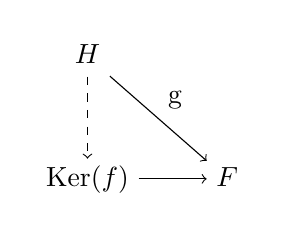
\begin{tikzpicture}[baseline=(current bounding box.center)]
        \matrix (m) [matrix of math nodes, row sep=3em, column sep=2.5em, text height=1.5ex, text depth=0.25ex] {
          H & \\
          \Ker(f) & F \\
        };
        \path[->] (m-1-1) edge node [auto] {g} (m-2-2);
        \path[->] (m-2-1) edge (m-2-2);
        \path[->,dashed] (m-1-1) edge (m-2-1);
      \end{tikzpicture}
    \end{equation}
  \end{quote}

  \begin{solution}
    The factorization is uniquely determined by~$g$, as it will map the sheaf~$G$ into~$\Ker(f)$ in a unique (namely its own) way.
  \end{solution}
\end{exercise}

\clearpage

\chapter{Solutions to the exercises at the end of Chapter 3}
\begin{enumerate}
  \item Let~$P$ be the category of pointed sets, whose objects are the pairs~$(A,a)$ with~$a\in A\in\Ob(\Sets)$, and whose morphisms $(A,a)\to(B,b)$ are the maps of sets~$f\colon A\to B$ such that~$f(a)=b$. Show that~$P$ is a category with a zero object, kernels and cokernels, but in which not every epimorphism is a cokernel.

    \begin{solution}
      Every singleton set~$(\left\{ x \right\},x)$ is a zero object. The initial object~$\emptyset$ from~$\Sets$ is now changed to~$(\left( x \right),x)$ as every morphism needs to map the base point. The terminal object~$\left\{ x \right\}$ in~$\Sets$ remains unchanged as it allows for exactly one morphism (which preserves the base point).

      For kernels and cokernels we need a zero morphism, which in this case is the projection on the base point. For a map~$f\colon(A,a)\to(B,b)$ we have that~$\Ker(f)=(f^{-1}(b),a)$ and~$\Coker(f)=(f(A),b)$.

      TODO
    \end{solution}

  \item For~$X$ any topological space, show that the following presheaves of sets over~$X$ are in facts sheaves:
    \begin{enumerate}
      \item\label{enumerate:exercise-2-a} Fixing an open~$V\subseteq X$, let
        \begin{equation}
          h_V(U)=
          \begin{cases}
            \text{singleton} & U\subseteq V \\
            \emptyset & U\nsubseteq V
          \end{cases}
        \end{equation}
        for~$U$ open in~$X$, with the unique restrictions.

        \begin{solution}
          Both the monopresheaf and the gluing condition are meaningless for~$U\nsubseteq V$, so they trivially hold. For~$U\subseteq V$ both conditions are valid as there is only one possible section. Therefore all restrictions and gluings are well-defined.
        \end{solution}

      \item\label{enumerate:exercise-2-b} Let~$\Omega(U)=\left\{ W\,|\,\text{$W\subseteq X$ open and~$W\subseteq U$} \right\}$ for~$U$ open in~$X$ with restriction: $\Omega(U)\to\Omega(V):W\mapsto W\cap V$. Interpreting presheaves on~$X$ as contravariant set-valued functors on~$\mathcal{U}$, the category of open sets of~$X$, show that the $h_V$ defined by~\ref{enumerate:exercise-2-a} are the representable functors
        \begin{equation}
          h_V=\Hom_{\mathcal{U}}(-, V)\colon U\mapsto\Hom_{\mathcal{U}}(U,V).
        \end{equation}

        \begin{solution}
          First of all note that~$\Omega(U)$ describes the (open) subspace topology induced by~$X$ on~$U$. Now we have in any topology (which is just a lattice) that
          \begin{equation}
            \Hom_{\mathcal{U}}(U,V)=
            \begin{cases}
              \left\{ \inj\colon U\hookrightarrow V \right\} & U\subseteq V \\
              \emptyset & U\nsubseteq V
            \end{cases}
          \end{equation}
          which corresponds to~$h_V=\Hom_{\mathcal{U}}(-,V)$.
        \end{solution}
    \end{enumerate}

    Interpret the Yoneda lemma as saying that
    \begin{equation}
      \Hom_{\PCat/X}(h_V,F)\overset{\simeq}{\to}F(V)
    \end{equation}
    for any presheaf~$F$ on~$X$. Putting~$F=h_U$, this shows that~$V\mapsto h_V$ is a full and faithful embedding of~$\mathcal{U}$ into~$\PCat/X$.

    \begin{solution}
      We have that~$\mathcal{U}$ is locally small (as each set of homomorphisms contains either zero or one morphism, which is quite small), so by the (contravariant) Yoneda lemma we can assign to each object~$V\in\mathcal{U}$ a functor~$h_V=\Hom(-,V)$ to~$\Sets$.
      
      Now we have that for each object~$V\in\mathcal{U}$ the natural transformations from the presheaf (of representable functor)~$h_V$ to a presheaf~$F$ (which is just a functor, we are working in an functor category) correspond bijectively to~$F(V)$. \Ie,
      \begin{equation}
        \Hom_{\PCat/X}(h_V,F)\overset{1:1}{\longleftrightarrow}F(V)
      \end{equation}
    \end{solution}

  \item For a topological space~$X$, let respectively~$\PCat/X$ and~$\SCat/X$ be the categories of presheaves and sheaves of sets over~$X$. Imitate the results of Chapter~$3$ as follows:
    \begin{enumerate}
      \item Show that~$F\to G$ is a monomorphism in~$\PCat/X$ (or in~$\SCat/X$) if and only if for all open~$U$ we have~$F(U)\to G(U)$ injective if and only if for all~$x\in X$ we have~$F_x\to G_x$ injective.

        \begin{solution}
          \begin{description}
            \item[$1\Rightarrow 2$] Presheaf morphisms are given by the morphisms on all open~$U$, so if~$f\in\Hom_{\PCat/X}(F,G)$ is a monomorphism, all maps between the sets of functions must be monomorphic in~$\Sets$.
            \item[$2\Rightarrow 1$] Trivial.
            \item[$2\Rightarrow 3$] We have that~$\varinjlim$ is exact, so the exactness of~$0\to F(U)\to G(U)$ is preserved.
            \item[$3\Rightarrow 2$] TODO
          \end{description}
        \end{solution}

      \item Show that~$F\to G$ is an epimorphism in~$\PCat/X$ if and only if for all open~$U$ we have~$F(U)\to G(U)$ is surjective, while~$F\to G$ is an epimorphism in~$\SCat/X$ if and only if for all~$x\in X$ we have~$F_x\to G_x$ surjective.
        
        \begin{solution}
          TODO

          For~$\SCat/X$, we have that~$g\circ f=h\circ f$ if and only if~$(g\circ f)_x=(h\circ f)_x$ on the stalks. Now $f$ is an epimorphism in~$\SCat/X$ if and only if the induced maps on the stalks are epimorphisms in~$\Sets$, and epimorphisms in~$\Sets$ are exactly the surjective maps.
        \end{solution}

      \item Discover an appropriate definition of ``equivalence relation''~$\sim$ on a presheaf~$F$ so that you can define a presheaf~$F/\sim$ (respectively a sheaf~$F/\sim$ if~$F$ is a sheaf) together with an epimorphism~$F\to F/\sim$ (in the appropriate category) with a universal property.

        \begin{solution}
          TODO
        \end{solution}

      \item Show that each of the categories~$\PCat/X$ and~$\SCat/X$ has all limits and all colimits (in particular all equalisers and coequalisers); that in each category every monomorphism is an equaliser and every epimorphism is a coequaliser; and that every morphism has a unique epimorphism-monomorphism factorisation.

        \begin{solution}
          TODO
        \end{solution}

      \item Show that for a continuous map~$\phi\colon X\to Y$ there are induced functors~$\SCat/X\overset{\phi_*}{\underset{\phi^*}{\rightleftarrows}}\SCat/Y$ (as in~\S~3.7) with the adjointness property~7.13 and such that~$\phi^*$ preserves all finite limits (analogue of~``$\phi^*$ is left exact'').

        \begin{solution}
          TODO
        \end{solution}

      \item Is there an analogue of extension by zero?

        \begin{solution}
          TODO
        \end{solution}
    \end{enumerate}

  \item Let~$F,G$ be presheaves of sets on a topological space~$X$. Define a new presheaf~$\uHom(F,G)$ with
    \begin{equation}
      \uHom(F,G)(U)\colonequals\Hom_{\Sets}\left( F(U),G(U) \right)
    \end{equation}
    for~$U$ open in~$X$. Show that if~$F$ and~$G$ are both sheaves, then so is~$\uHom(F,G)$.

    \begin{solution}
      \begin{description}
        \item[$\uHom(F,G)$ presheaf] By restricting a section~$f\in\uHom(F,G)(U)$ to its restriction~$\restr_V^U(f)$ we get by commutativity in the diagram for sheaf morphisms a good section in~$\uHom(F,G)(V)$, compatible with all restrictions, for~$V\subseteq U$ open.
        \item[$\uHom(F,G)$ monopresheaf] Given the situation for the monopresheaf condition, if~$s\neq s$, both being maps~$F(U)\to G(U)$ they must disagree on some~$x\in U$, \ie, $s(u)\neq s(u')$. But~$u\in U_\lambda$ for some~$\lambda\in\Lambda$, so~$\restr_{U_\lambda}^U(s)(x)\neq\restr_{U_\lambda}^U(s')(u)$, a contradiction.
        \item[$\uHom(F,G)$ glues] Define the section over~$U$ by its values in the~$U_\lambda$, the obvious restrictions are satisfied and we get a section glued from its components.
      \end{description}
    \end{solution}

    Prove that this construction has the following universal property: for~$F$,~$G$,~$H$ presheaves (respectively sheaves) of sets on~$X$, there is a bijection
    \begin{equation}
      \Hom\left( H,\uHom(F,G) \right)\cong\Hom\left( H\times F,G \right)
      \label{equation:natural-bijection}
    \end{equation}
    natural in~$F$,~$G$ and~$H$. Here~$H\times F$ is the product object provided by~3(d); it is constructed ``pointwise''.

    \begin{solution}
      Take~$\mathcal{F}\in\Hom(H,\uHom(F,G))$, that is for~$U\subseteq X$ open we have
      \begin{equation}
        \sections(U,\mathcal{F})\colon
        \begin{array}{ccc}
          H(U)&\to &\uHom(F,G)(U)=\Hom_{\Sets}\left( F(U),G(U) \right) \\
          h&\mapsto & \left( f_h\colon F(U)\to G(U):x\to f_h(x) \right).
        \end{array}
      \end{equation}
      This is now mapped to~$\Hom(H\times F,G)$ by mapping each~$\sections(U,\mathcal{F})$ to the map
      \begin{equation}
        \begin{array}{ccc}
          \left( H\times F \right)(U)=H(U)\times F(U)&\to&G(U) \\
          (h,f)\mapsto\mathcal{F}(h)(f)
        \end{array}
      \end{equation}

      \begin{description}
        \item[surjectivity] We can uniquely define an~$\mathcal{F}\in\Hom(H,\uHom(F,G))$ by this construction, so the map is surjective. In more detail, define
          \begin{equation}
            \sections(U,\mathcal{F})\to
            \begin{array}{ccc}
              H(U)&\to&\uHom(F,G)(U) \\
              h&\mapsto& \left( f\mapsto g \right)
            \end{array}
          \end{equation}
          and this provides a good preimage.
        \item[injectivity] Assume~$\mathcal{F}_1$ and~$\mathcal{F}_2$ in~$\Hom(H,\uHom(G,F))$ are mapped to the same element in~$\Hom(H\times F,G)$. Then by the construction above the inverse image of this element corresponds to a unique element in the domain, a contradiction.
      \end{description}
    \end{solution}

    Show that, if we want the property~\eqref{equation:natural-bijection} to hold, then the definition of~$\uHom$ is forced on us, for presheaves at least.

    \begin{solution}
      TODO
    \end{solution}

    Reinterpret~\eqref{equation:natural-bijection} as requiring the existence of an evaluation map
    \begin{equation}
      \uHom(F,G)\times F\to G
    \end{equation}
    with a suitable universal property.

  \item 

  \item Since any category of presheaves is a functor category, we can define it for categories other than those of open sets of a topological space. For~$\mathcal{C}$ any category, let~$\PCat/\mathcal{C}$ be the category~$\Sets^{\mathcal{C}^{\opp}}$ of contravariant functors~$\mathcal{C}\to\Sets$ (and natural transformations).

    As a special case, any group~$G$ can be regarded as a category with one object whose endomorphisms are the elements of~$G$, with composition defined as in~$G$ (hence every morphism is an isomorphism). Show that the category~$\PCat/G$ can be regarded as the category of sets-with-a-$G^{\opp}$-action, that is the category of permutation representations of~$G$.

    \begin{solution}
      As~$F\in\PCat/G$ is a contravariant functor~$G\to\Sets$ and by definition of the category of a group~$\Ob(G)=\left\{ \cdot_G \right\}$, we have~$F(\cdot_G)$ a set. As all endomorphisms defined on~$\cdot_G$ by~$G$ are invertible ($G$ a group, not just a monoid) we have~$F(\End(\cdot_G))=\Aut\left( F(\cdot_G) \right)$, \ie, all bijections or permutations on~$F(\cdot_G)$. Now every~$g\in G$ defines an (invertible) action on the set~$F(\cdot_G)$, in which~$x\in F(\cdot_G)$ is mapped to~$F(\cdot_G)(x)$.
    \end{solution}

  \item If~$\mathcal{A}$ and~$\mathcal{B}$ are abelian categories, a functor~$F\colon\mathcal{A}\to\mathcal{B}$ is called \emph{half exact} if and only if whenever~$0\to P\to Q\to R\to 0$ is exact in~$\mathcal{A}$, $F(P)\to F(Q)\to F(R)$ is exact in~$\mathcal{B}$. $F$ is called \emph{additive} if and only if all the maps~$F\colon\Hom_{\mathcal{A}}(P,Q)\to\Hom_{\mathcal{B}}(F(P),F(Q))$ are abelian group homomorphisms.

    Consider the conditions
    \begin{enumerate}
      \item\label{enumerate:additive-1} $F$ is half exact;
      \item\label{enumerate:additive-2} $F$ preserves biproducts;
      \item\label{enumerate:additive-3} $F$ is additive.
    \end{enumerate}
    Show that~$\ref{enumerate:additive-1}\Rightarrow\ref{enumerate:additive-2}\Leftrightarrow\ref{enumerate:additive-3}$.

    \begin{solution}
      \begin{description}
        \item[$\ref{enumerate:additive-1}\Rightarrow\ref{enumerate:additive-2}$] We show
        \item[$\ref{enumerate:additive-1}\Rightarrow\ref{enumerate:additive-2}$]<++>
        \item[$\ref{enumerate:additive-1}\Rightarrow\ref{enumerate:additive-2}$]<++>
      \end{description}<++>
    \end{solution}<++>

  \item 

  \item 

  \item A sheaf~$F$ of abelian groups on~$X$ is called \emph{locally free} if and only if each point~$x\in X$ has an open neighbourhood~$U$ in~$X$ such that the sheaf~$F|_U$ is isomorphic to a constant sheaf with typical stalk a free abelian group (of finite rank). Show that if~$X$ is connected, a locally free sheaf has a well-defined rank.

    \begin{solution}
      TODO
    \end{solution}

    Show by example that a locally free sheaf on~$X$ need not be isomorphic to a constant sheaf even if~$X$ is connected, and that~$\phi_*$ does not preserve the property of being locally free.

    \begin{solution}
      Take~$X=\left\{ 0,1,2 \right\}$ with topology~$\mathcal{T}=\left\{ \left\{ 0,1 \right\},\left\{ 1 \right\},\left\{ 1,2 \right\},X \right\}$ and define~$F$ to be the sheaf with sections
      \begin{align}
        \sections\left( \left\{ 0,1 \right\},F \right)&=\mathbb{Z} \\
        \sections\left( \left\{ 1,2 \right\},F \right)&=\mathbb{Z} \\
        \sections\left( \left\{ 1 \right\},F \right)&=\mathbb{Z} \\
        \sections\left( \left\{ 0,1,2 \right\},F \right)&=\mathbb{Z}\oplus\mathbb{Z}
      \end{align}
      with restriction morphisms the projection on the first term. Now take for~$x\in X$ any open~$U\neq X$, then~$F|_U=U_\mathbb{Z}$, but~$F$ is not isomorphic to any constant sheaf.
      

    \end{solution}

    Prove however that the inverse image of a locally free sheaf of rank~$n$ is locally free and of the same rank.

    \begin{solution}
      TODO
    \end{solution}
\end{enumerate}

\end{document}
